\section{Hyperbolic Functions}
\begin{itemize}
    \item Sometimes, combinations of $e^x$ and $e^{-x}$ are given certain names, for example:
    \begin{itemize}
        \item \textbf{Hyperbolic sine:} $\sinh(x) = \frac{1}{2}(e^x-e^{-x})$
        \item \textbf{Hyperbolic cosine:} $\cosh(x) = \frac{1}{2}(e^x+e^{-x})$
    \end{itemize}
    \item They have the following properties:
    \begin{align}
        \frac{d}{dx} \sinh x &= \cosh x \\ 
        \frac{d}{dx} \cosh x &= \sinh x
    \end{align}
    \item They are related via:
    \begin{equation}
        \cosh^2 x - \sinh^2 x = 1
    \end{equation}
    \item Both the area of a circular sector and that of a hyperbolic sector is described by:
    \begin{equation}
        A = \frac{1}{2}t
    \end{equation}
    where $t$ is the subtended angle, and the figures are parametized by $(\cos t, \sin t)$ and $(\cosh t, \sinh t)$.
    \begin{center}
        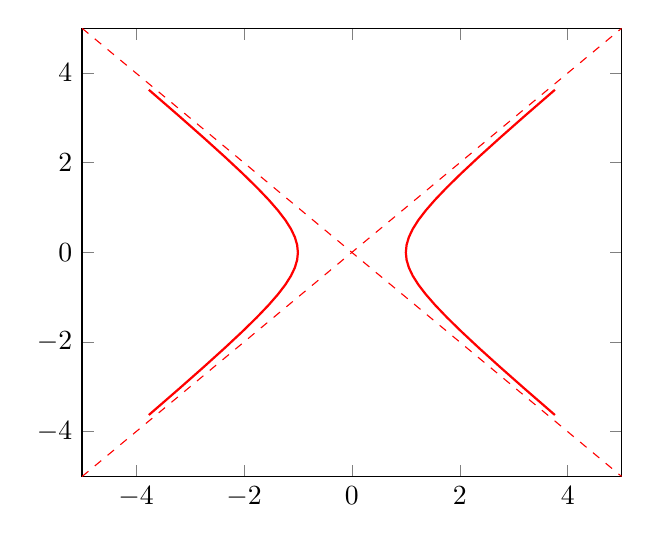
\begin{tikzpicture}
            \begin{axis}[
                    xmin=-5,xmax=5,
                ymin=-5,ymax=5]
                \addplot [red,thick,domain=-2:2] ({cosh(x)}, {sinh(x)});
                \addplot [red,thick,domain=-2:2] ({-cosh(x)}, {sinh(x)});
                \addplot[red,dashed] expression {x};
                \addplot[red,dashed] expression {-x};
            \end{axis}
        \end{tikzpicture}
        \begin{tikzpicture}
            \begin{axis}[
                    xmin=-2,xmax=2,
                ymin=-2,ymax=2]
                \addplot [domain=-180:180, samples=1000, red, thick] ({cos(x)},{sin(x)});
            \end{axis}
        \end{tikzpicture}
    \end{center}
    \item The catenary
    \begin{equation}
        y = a\cosh\left(\frac{x}{a}\right)+C
    \end{equation}
    describes the shape of a free hanging rope between two walls separated by a width $a$.
    \item The hyperbolic tangent is given by $\tanh x = \frac{\sinh x}{\cos h x} = \frac{e^x-e^{-x}}{e^x+e^{-x}}$. and its derivative is given by:
    \begin{equation}
        \frac{d}{dx} \tanh x = \sech^2x
    \end{equation}
    \item The inverse of $y=\sinh x$ is given by:
    \begin{equation}
        \sinh^{-1}x = \ln\left(x+\sqrt{x^2+1}\right)
    \end{equation}
    \begin{tip}
        A table of integrals and derivatives revolving around hyperbolic trig functions can be found in the textbook.
    \end{tip}
\end{itemize}